\section*{Discussion}
\label{sec:discussion}

That \ac{NSC} can explain and reproduce response properties 
observed in biological neurons 
may be an important clue as to how 
\revise{sensory and associative brain areas}
have evolved to parse and store information
in order to perceive the world and interact with it.
\mikeNote{This is indeed written in a very sensory-centric manner}
We offer three testable predictions of this theory:

First, we suggest that a variety of neuronal response properties
can be understood as an emergent property of efficient population coding 
based on dimensionality reduction.
Depending on input stimulus and task complexity,
we expect the dimensionality of the population code to be adjusted
according to the bias-variance dilemma
(Fig.~\ref{fig:nsc-bias-variance-dilemma}).
This point of operation might differ across brain areas---for example,
favoring neurons that respond to a small number of stimulus dimensions
in \ac{V1} \cite{OlshausenField1996},
but giving rise to mixed selectivity in higher-order brain areas
such as \ac{MSTd} \cite{Beyeler2016} and
\ac{RSC} \cite{Rounds2016,Rounds2018}.
% and \ac{PFC} \cite{Mante2013}.

Second, we predict that parts-based representations can explain
\acp{RF} of neurons in a variety of brain regions,
including but not limited to those brain areas discussed here. 
In agreement with the literature on basis function representations
\cite{PougetSejnowski1997,PougetSnyder2000,Poggio1990},
we expect parts-based representations
to be prevalent in regions where neurons
exhibit a range of tuning behaviors \cite{Beyeler2016},
display mixed selectivity \cite{Fusi2016,Eichenbaum2017},
or encode information in multiple reference frames 
\cite{AlexanderNitz2015,Rounds2016,Rounds2018}.

Third, where such representations occur, we expect the resulting
neuronal population activity to be relatively sparse,
in order to encode information both accurately and efficiently.
As noted above, sparse codes offer a trade-off between 
dense codes (where every neuron is involved in every context,
leading to great memory capacity but suffering from cross talk among neurons)
and local codes (where there is no interference, 
but also no capacity for generalization).


% \subsection*{\revise{Potential for NSC in nonsensory areas of the brain}}

% % \revise{Complex behaviors are accompanied by dynamic responses across cortical circuits.
% % During decision-making, cortical activity reflects multiple processes including sensory inputs (Freedman and Assad, 2006; Meister et al., 2013), selection and integration of behaviorally-relevant information (Roitman and Shadlen, 2002), estimation and anticipation of reward (Bouret and Sara, 2004; Pratt and Mizumori, 2001), choice confidence (Kepecs et al., 2008) and recent trial history (Abrahamyan et al., 2016; Bichot and Schall, 1999; Manoach et al., 2007; Morcos and Harvey, 2016).} 

% \mikeNote{Maybe fuse with model limitations?}
% \mikeNote{R1: In the previous round of reviews, I already suggested that the authors’ model seems more appropriate for sensory areas, and that it may not apply to the motor system. Despite the changes to the paper, I think the paper would be clearer and perhaps more compelling that way. To be clear, I’m not arguing that the authors should complete remove non-sensory areas, but I think it should be a part of the Discussion ``Would these ideas apply to non-sensory areas?'' rather than of the core of the paper.}
% \revise{In addition to the areas highlighted above,
% there is increasing evidence that the essential components of \ac{NSC}
% might be present in numerous brain regions 
% not traditionally associated with the efficient encoding of information.}

% \emilyNote{Should discussion of hippocampus go here?}

% \revise{For example, there is evidence for sparse coding in the
% cerebellum \cite{Marr1969,Schweighofer2001,Brunel2004},
% \ac{PFC} \cite{Abeles1990,Fujisawa2008,Wei2015},
% motor cortex \cite{Beloozerova2003,Kakei2003,BarthPoulet2012,Brecht2004},
% hippocampus \cite{rolls2013,ThompsonBest1989,Poli2017,Wixted2014},
% and the amygdala \cite{Bach2011}.
% Similarly, there is evidence for dimensionality reduction in
% \ac{PFC} \cite{Mante2013}
% and motor cortex \cite{Graziano2009,Gallego2017}.
% However, the intrinsically complex response properties of individual neurons
% have defied a deep understanding of how these neurons contribute to behavior
% \cite{churchland2007,Mante2013}.
% For example, individual \ac{PFC} neurons typically encode multiple task-related signals
% at once, including the animal's upcoming choice, the context,
% and the strength of the sensory evidence \cite{Mante2013,Rigotti2013,Kobak2016}.
% Future studies may show that key features of the population response in these regions
% can be recovered by applying \ac{NSC} to their inputs.}

% \revise{Analogous to our modeling work in \ac{MSTd} \cite{Beyeler2016},
% it might be possible to apply \ac{NSC} to other areas of the posterior parietal
% cortex that are involved in multisensory heading perception.
% Areas such as the \ac{VIP} and \ac{VPS} are also known to respond to optic flow,
% but they increasingly respond to inertial vestibular stimulation as well
% \cite{Chen2011}.
% Although the degree of sparsity of the population code in \ac{VIP} and \ac{VPS} is not known,
% the fact that neurons in these areas respond to mixtures of visual and vestibular
% heading cues make them prime examples 
% to be examined with an \ac{NSC} based modeling approach.}

% \revise{Elsewhere in parietal cortex, single neurons act as basis functions 
% to represent the spatial configuration of objects 
% with respect to multiple reference frames
% (e.g., by transforming eye-centered to body-centered coordinates).
% \cite{Poggio1990,PougetSejnowski1997,PougetSnyder2000}.
% This is similar to the integration of multimodal heading cues mentioned above,
% as well as to other associative areas such as \ac{RSC},
% which demonstrates conjunctive coding of various spatial navigation cues
% \cite{AlexanderNitz2015,Rounds2018}.
% There is further evidence that actions are represented in parietal cortex
% with respect to arbitrary and abstract reference frames, 
% such as with respect to a planned route through an environment \cite{nitz2009parietal}.
% From a theoretical standpoint, \ac{NSC} seems a good candidate to find an efficient,
% reference-frame agnostic representation of various behaviorally relevant variables
% \cite{LouieGlimcher2012,louie2015adaptive,andersen1997multimodal,BenHamed2003},
% but future studies will have to address these issues step by step.}


\subsection*{Potential neural mechanisms of NSC}

As a special case of efficient coding,
\mikeNote{I'm not really sure what to do with this section. If we remove the energy efficiency stuff here, there's only one paragraph left, and it kinda sticks out. Plus it offers just one potential neural mechanism.}
\mikeNote{R1: minimizing energy expenditure is not a clear requirement for the NSC model to be useful; maybe some areas try to maximize robustness or adaptability instead of miniziming energy expenditure. maybe that's why some areas are less sparse than others.}
\ac{NSC} possesses metabolic advantages by employing
sparse population codes.
To operate efficiently, it has been suggested that the brain might enforce 
geometrical and biophysical constraints on axonal wiring 
\cite{LaughlinSejnowski2003}.
In addition to reducing overall wiring length
\cite{Cherniak1994}, the brain might also aim to minimize local delays
by favoring a high degree of local connectivity
\cite{Chklovskii2002}.
\revise{If connectivity reflects} coding \cite{Clopath2010},
it would not be surprising to find that such ecological considerations
carry over into brain function,
favoring sparse population codes and neuronal representations that are
local in functional space (i.e., parts-based).
However, wiring cost is likely to be only one of many constraints 
on the brain connectome, perhaps supplementing competitive pressures
for hub-mediated information exchange between network modules
\cite{Rubinov2015}.

In addition, evidence suggests that Hebbian-like synaptic plasticity rules
allow neurons to perform statistical inference on their inputs
\cite{Nessler2009,Carlson2013,MorenoBoteDrugowitsch2015,Oja1982}.
One particular study demonstrated through a mathematical proof
that a certain form of \textbf{\ac{STDP}} in combination with 
homeostatic synaptic scaling (i.e., \ac{STDPH})
can approximate the \ac{NMF} algorithm
\cite{Carlson2013}.
Similar to Oja's rule \cite{Oja1982}, which was developed to stabilize 
rate-based Hebbian learning
(effectively resulting in principal component analysis),
Carlson and colleagues showed that synaptic scaling acts as a 
homeostatic mechanism to stabilize \ac{STDP}
(effectively resulting in \ac{NMF}).
Interestingly, we were able to apply these ideas to 
electrophysiologically recorded neuronal activity observed in the \ac{RSC}
of rats during a spatial navigation task (Fig.~\ref{fig:NMF|RSC}; for experimental details see Supplementary Material). Both \ac{STDPH} and \ac{NMF} were able to recover key  features such as encoding spatial reference frames (i.e., allocentric and route-centric firing patterns) and position discrimination by reducing the dimensionality of behavioral variables (e.g., velocity, head direction, position).
The neuronal and population responses from NMF and STDPH were comparable to the experimental findings \cite{AlexanderNitz2015}.
Furthermore, the \ac{STDPH} model contained a highly flexible and generalizable code
that could automatically encode new routes through the same environment
without retraining \cite{Rounds2018}.

However, more research is needed to elucidate any potential connection 
between \ac{NSC} and the many different synaptic plasticity rules 
commonly found across brain regions,
different stages in the life of an animal, and animal species
(e.g., \cite{Froemke2010,BCM1982}).
\mikeNote{R1:  Fig 8 is hard to interpret, what is the percent model error? Does this error reflect a ``movement prediction error''?}
\mikeNote{For R1: Fig.8 caption needs a sentence about what the error bars mean. Why are alphas and betas low in prediction error? Why are alphabetas not?}
\begin{figure}[h]
	\centering
	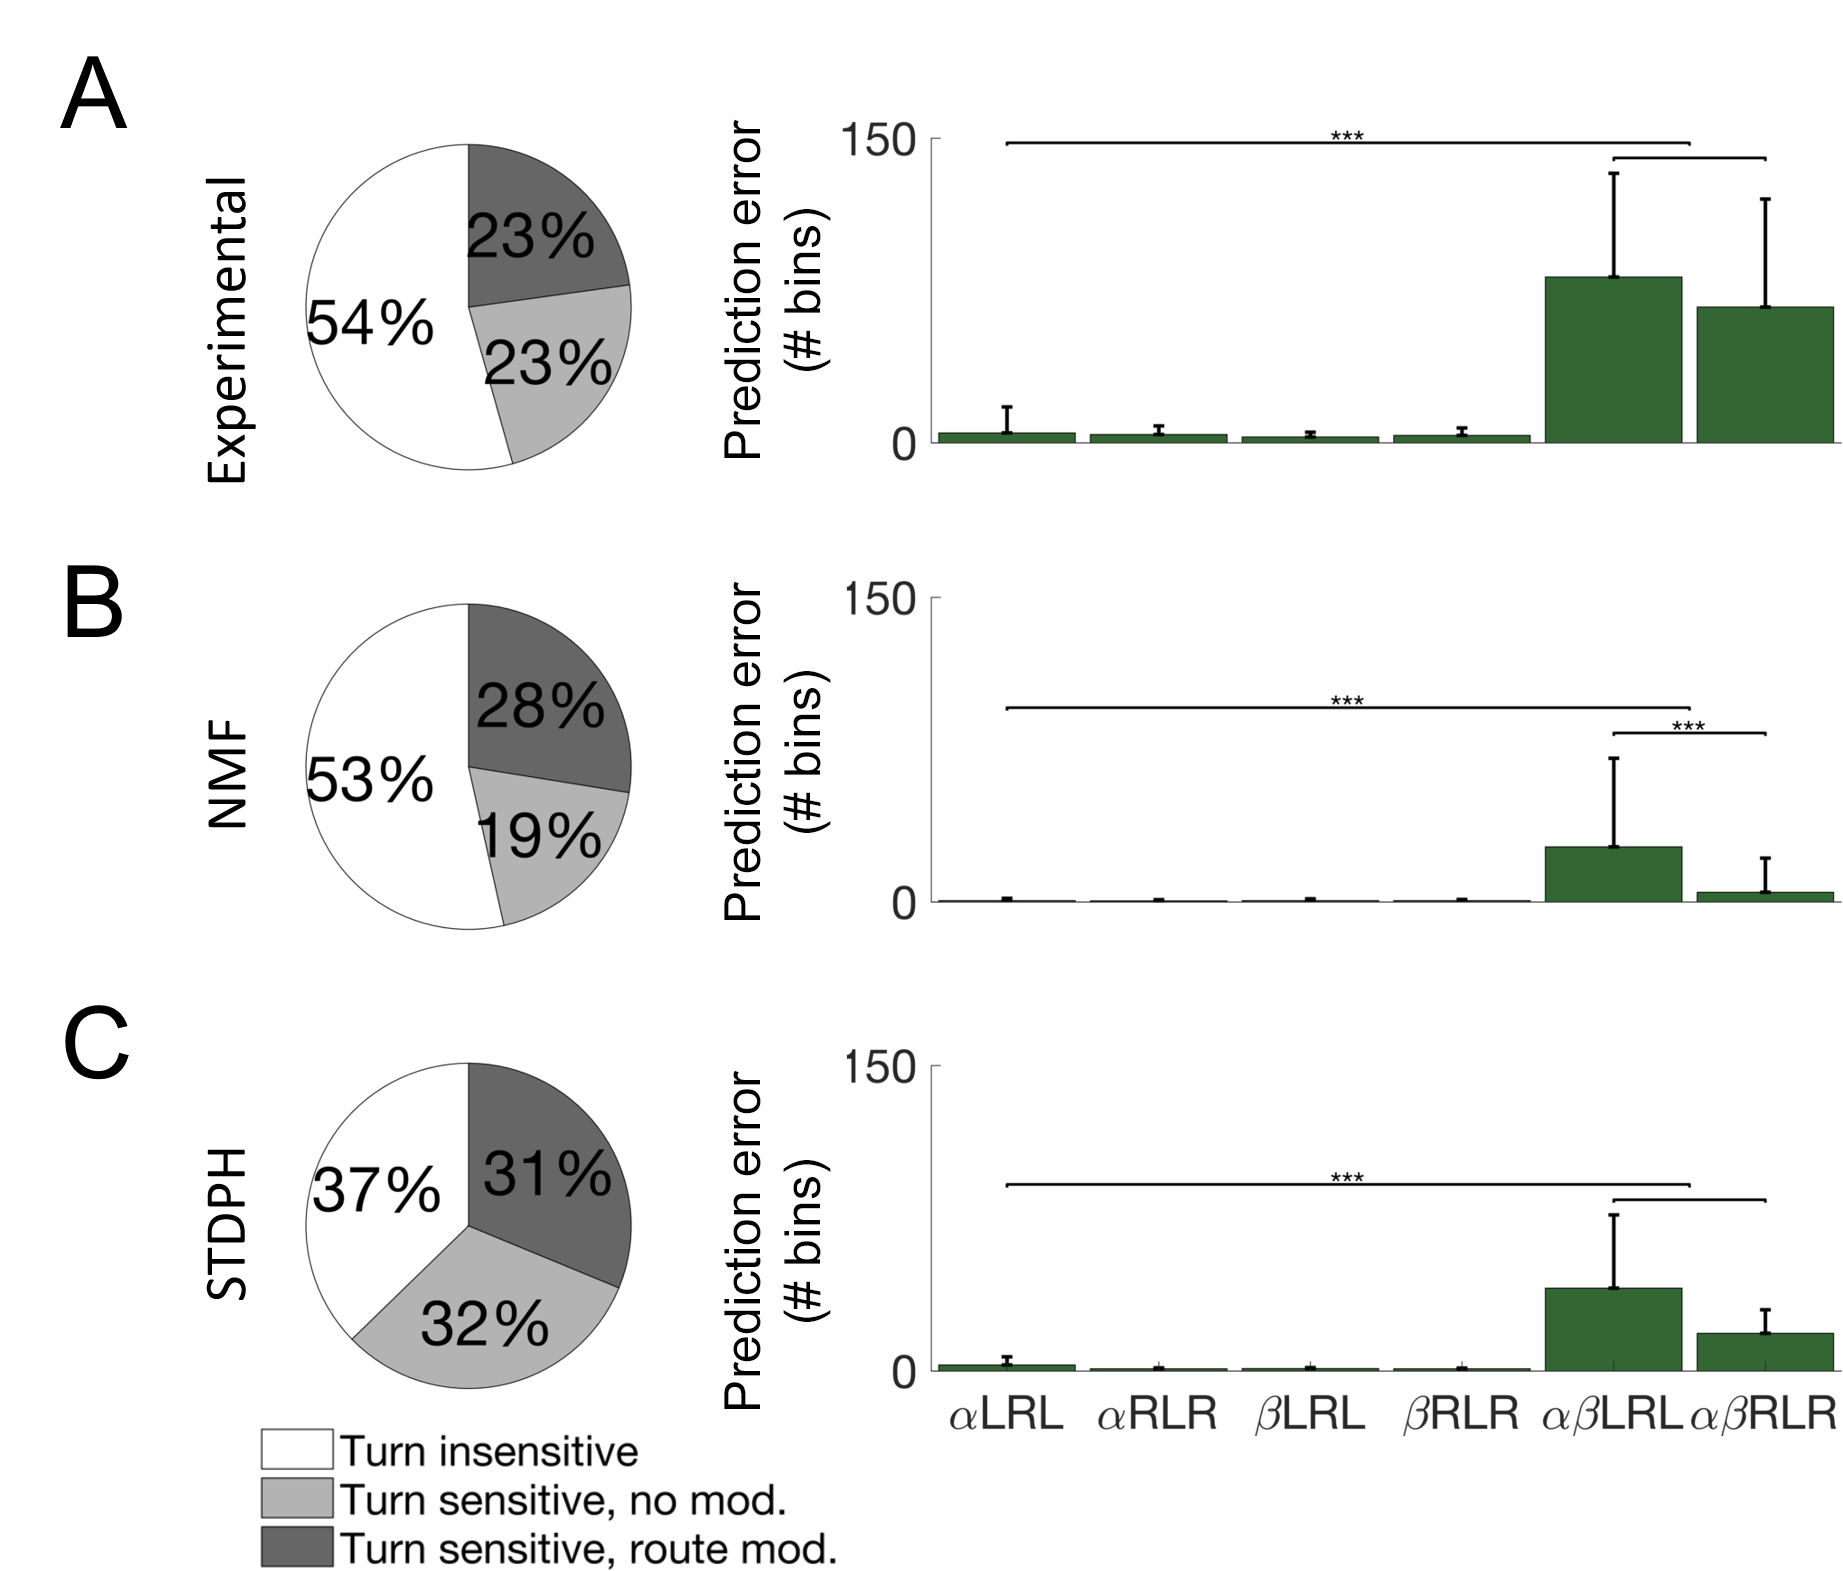
\includegraphics[width=0.95\textwidth]{fig-rev2-rsc}
    \caption{
    	Comparisons between recorded experimental data and two 
        computational models of rat \ac{RSC} suggest a functional 
        similarity between \ac{STDPH} and \ac{NMF}.
%         (adapted \revise{with permission} from \cite{Rounds2018}). 
        Using methods described in \cite{AlexanderNitz2015}, 
        we compared functional neuron type distributions (left column)
        and average \revise{movement} prediction errors (right column)
        observed \emph{in vitro} (\textbf{\emph{A}}) with those
        produced by each model (\textbf{\emph{B, C}}).
        Average error corresponded to correlation matrices 
        representing reconstructed position within a route. 
        For details, see Supplementary Materials.
        Separate positions of the W-shaped track are represented 
        by the symbols $\alpha$ and $\beta$. 
        Outbound and inbound runs were made up of 
        opposite turn sequences (left-right-left (LRL) 
        and right-left-right (RLR), respectively.
        Reconstructions between the track positions are represented by
        $\alpha \beta$.
	    \textbf{\emph{A}},
    		Experimental data from \cite{AlexanderNitz2015}.
        \textbf{\emph{B}},
            Simulated using NMF with sparsity constraints.
        \textbf{\emph{C}},
            Simulated by evolving \ac{STDPH} parameters 
            to fit experimental data \cite{BeyelerCarlsonChou2015,Carlson2014}.
    }
	\label{fig:NMF|RSC}
\end{figure} 



\subsection*{\revise{Would these ideas apply to nonsensory brain areas?}}

\mikeNote{R1 specifically asked for this section. I think it makes sense here - could we extend the theory to other brain areas? Then limitations talks about all the drawbacks or shortcomings of NSC. Sound good?}
\revise{NSC is clearly better suited for sensory and associative areas, where there's a clear definition of the input or stimulus space a neuronal population might be encoding. It is difficult to think about what parts-based means for more complicated regions.}
\mikeNote{informal intro but summing up reviewers rant, revise}

\revise{For example, studies indicate that the population code in \ac{PFC} and \ac{M1} 
may be quite dense (as in Fig.~\ref{fig:sparse-parts}A).
Moreover, dimensionality reduction studies in these regions suggest that 
features are encoded by most neurons in the population, 
rather than a sparse parts-based representation 
\cite{Gallego2017,CunninghamYu2014,Kobak2016,Mante2013}. 
Furthermore, \ac{M1} neurons tend to be active during most movements, 
which argues against a sparse activation. 
This may be due to the role of the motor system, which is to cause behavior, 
rather than represent features.}

\revise{There are aspects of the hippocampus that are comparable to the ideas 
of \ac{NSC} proposed here.
For example, the dentate gyrus is often associated with sparse activity
\cite{GoodSmith2017,JungMcNaughton1993,SenzaiBuzsaki2017}.
The expansion from a dense, enthorhinal cortex coding to sparse dentate gyrus 
activity suggested a mechanism of pattern separation
\cite{Marr1971,TrevesRolls1994}.
Since these early theories, accumulating evidence has supported 
the role of the dentate gyrus in pattern separation 
\cite{GoodSmith2017,SenzaiBuzsaki2017,YassaStark2011}.
However, the dentate gyrus projects to a highly recurrent CA3 region, 
which does not appear to be sparse or reduce dimensionality. 
Rather, the CA3 region has a role in pattern completion through auto-association 
\cite{KnierimNeunuebel2016,Marr1971,TrevesRolls1994}.
Another feature of hippocampal processing that is related to \ac{NSC} 
may be the place cell itself.
Sparsity has long been used as a metric for place cell quality \cite{Skaggs1996}.
A place cell is said to be sparse if it fires in a small region of the environment, 
and this is related to how much spatial information that cell encodes. 
In a sense, each place cell can be thought of as a ``part'' of the environment 
and these parts cover the entire environment. 
Although this evidence points to sparse, parts-based, 
and reduced coding in some hippocampal regions, 
it does differ from the \ac{NSC} representations in sensory areas.
That is, sparse coding as defined above for sensory areas is not necessarily the same 
as sparsity or as sparse activity leading to pattern separation. 
Still, it would be of interest to apply \ac{NSC} to the hippocampal inputs, 
similar to the methods applied to \ac{RSC} 
during a spatial navigation task \cite{Rounds2018},
to see if sparse, reduced basis functions emerge in other regions.}

Analogous to our modeling work in \ac{MSTd} \cite{Beyeler2016},
it might be possible to apply \ac{NSC} to other areas of the posterior parietal
cortex that are involved in multisensory heading perception.
Areas such as the \ac{VIP} and \ac{VPS} are also known to respond to optic flow,
but they increasingly respond to inertial vestibular stimulation as well
\cite{Chen2011}.
Although the degree of sparsity of the population code in \ac{VIP} and \ac{VPS} is not known,
the fact that neurons in these areas respond to mixtures of visual and vestibular
heading cues make them prime examples 
to be examined with an \ac{NSC} based modeling approach.

Elsewhere in parietal cortex, single neurons act as basis functions 
to represent the spatial configuration of objects 
with respect to multiple reference frames
(e.g., by transforming eye-centered to body-centered coordinates).
\cite{Poggio1990,PougetSejnowski1997,PougetSnyder2000}.
This is similar to the integration of multimodal heading cues mentioned above,
as well as to other associative areas such as \ac{RSC},
which demonstrates conjunctive coding of various spatial navigation cues
\cite{AlexanderNitz2015,Rounds2018}.
There is further evidence that actions are represented in parietal cortex
with respect to arbitrary and abstract reference frames, 
such as with respect to a planned route through an environment \cite{nitz2009parietal}.
From a theoretical standpoint, \ac{NSC} seems a good candidate to find an efficient,
reference-frame agnostic representation of various behaviorally relevant variables
\cite{LouieGlimcher2012,louie2015adaptive,andersen1997multimodal,BenHamed2003},
but future studies will have to address these issues step by step.



\subsection*{Model limitations}

% sparse single-neuron responses underlying dense population codes are a common feature of cortical representations at the level of firing rates

Although \ac{NSC} has proved useful in understanding
a variety of neuronal responses
as an emergent property of efficient population
coding based on dimensionality reduction and sparse coding,
there are some limitations to this theory.

\revise{First, there is increasing evidence that several motor variables are encoded
throughout the brain, including early sensory areas 
\cite{CrochetPetersen2006,Pachitariu2015,Musall2018,Stringer2018}.
For example in the mouse, running modulates the gain of visual inputs 
\cite{Mineault2016,NiellStryker2010} 
and is critical for integration of visual motion \cite{Ayaz2013,Saleem2013}.
A potential explanation for these widespread effects is that 
certain movements reflect changes in the animal's internal state,
such as increased arousal during running \cite{NiellStryker2010}.
Another study found that stimuli and behavior 
were represented together in mouse \ac{V1} as a
mixed representation: there were not separate sets of neurons
encoding stimuli and behavioral variables, but each
neuron multiplexed a unique combination of sensory and
behavioral information \cite{Stringer2018}.
Interestingly, these results were not specific to visual cortex, but were seen across
wide regions of the mouse forebrain,
suggesting that neuronal activity in these areas is more than just an efficient
encoding of sensory stimuli.}

Second, a practical limitation of dimensionality analyses in general
is that the apparent dimensionality of the population response changes
systematically with the complexity of the input stimulus
\cite{SpanneJorntell2015,Cowley2016,Mazzucato2016}.
For practical purposes, simulated models of neuronal circuitry are typically
built with far fewer units than the number of neurons in the real network.
By excluding input dimensions that are present in the brain,
one will implicitly guide the simulated model away from spurious interactions
that the real circuitry would have to handle.
As a result, the simulated model might underestimate 
the true complexity of the task.

Third, the role of sparse coding in the brain has been questioned
\cite{SpanneJorntell2015,BarthPoulet2012}.
This is at least partly due to the wide variety of definitions of \revise{sparsity}
used in the literature:
In its widest possible theoretical sense,
a neuron population exhibits sparse activity if the average activation ratio
remains below 50\% for binary neurons 
or below 100\% for thresholded,
rate-based neurons \cite{SpanneJorntell2015}.
However, it is not surprising that different brain areas might employ
different degrees of sparsity.
\mikeNote{R1: These paragraphs are not very clear, starting with the authors’ definition of learning... Please rewrite}
Whereas learning can be extremely fast in a local code,
a network of `grandmother' cells suffers from low representational capacity.
As the degree of sparsity in the network decreases and the code gets denser,
representational capacity and fault tolerance 
(i.e., the capacity to handle neuronal noise or the loss of a subset of neurons)
improve,
but at the expense of a decrease in learning speed
\cite{Foldiak1990,SpanneJorntell2015}.
The optimal point of operation would therefore depend on the complexity of
the stimulus to be encoded or the task to be performed,
subject to constraints on the required speed of learning.
This point of operation might differ drastically across brain areas---for example,
favoring an extremely sparse code in \ac{V1}
\cite{OlshausenField1996},
but giving rise to a slightly denser code with 
greater representational capacity in higher-order visual areas
such as \ac{MSTd}, 
which could lead to compact and multifaceted encodings
of various perceptual variables
(see Discussion in \cite{Beyeler2016}).


\subsection*{Model alternatives}

Since \ac{NMF} is an integral part 
of Eq.~\ref{eqn:nsc-cost-function},
it is interesting to note that \ac{NSC} is tightly connected
to a number of unsupervised learning techniques,
such as $k$-means clustering,
an algorithm used to partition
$n$ observations into $k$ clusters
\cite{Ding2005}.
Due to its ability to decompose high-dimensional data into
sparse, interpretable factors, \ac{NMF} has become a 
widely used tool for the analysis of high-dimensional data,
with applications reaching far beyond
the field of computational biology
(for a recent review see \cite{Gillis2014}).

In addition to the tight connection 
to linear sparse coding and \ac{NMF}
\cite{EggertKorner2004},
\ac{NSC} is also intimately related to \textbf{\ac{ICA}},
a computational method for separating a multivariate signal
into additive, statistically independent subcomponents. 
As originally noted by Hoyer \cite{Hoyer2002},
if the fixed-norm constraint is placed on the rows of
\textbf{H} instead of the columns of \textbf{W},
Eq.~\ref{eqn:nsc-cost-function} can be directly interpreted as the joint
log-posterior of the basis functions and hidden components
in the noisy \ac{ICA} model \cite{HoyerHyvarinen2002}.
In order for this connection to hold,
the \ac{ICA} basis functions must be chosen to be nonnegative,
and the independent components must have 
exponential distributions \cite{Hoyer2002}.

Similarly, \ac{NSC} is closely related to compressed sensing
(for a recent review see \cite{GanguliSompolinsky2012}),
and a recent study has even suggested to combine the two
\cite{WangLi2010}.
Compressed sensing posits that neurons might implement 
dimensionality reduction by randomly projecting patterns of activity
into a lower-dimensional space,
simply by synaptically mapping $N$ upstream neurons to a downstream region
containing $M < N$ neurons. 
The theory of compressed sensing then provides the mathematical tools
to reconstruct the original space from the random projections.
\revise{Trautmann and colleagues \cite{trautmann2017} showed that this idea might apply to the motor system: When they applied random projection theory to data from three previous studies of motor area \ac{M1}, they found that the reconstructed neural dynamics yielded results quite similar to those derived from spike sorting.}

\ac{NSC}, \ac{ICA}, and compressed sensing often make similar predictions
that only slightly differ in the nature of the basis function representation
necessary to achieve optimal reconstruction
(for details please refer to the Discussion of \cite{GanguliSompolinsky2012}).
For example, whereas \ac{ICA} emphasizes the statistical independence 
of unmixed sources
and compressed sensing requires basis function to be `maximally incoherent'
\cite{GanguliSompolinsky2012},
\ac{NSC} does not make any such assumptions
as long as the basis functions are nonnegative.



